\documentclass{packages/labsec_planos}  
%\usepackage[utf8]{inputenc}
%\usepackage[T1]{fontenc}
%\usepackage[brazil]{babel}
%\usepackage{longtable}
%\usepackage{colortbl}
%\usepackage[a4paper]{hyperref}
%\usepackage{indentfirst}
%\usepackage{cite}
% Para codigo fonte %

\usepackage{listings}
%\usepackage{wrapfig}
\usepackage{nomencl}

%%%%%%%%% COLOCA MARCA D'AGUA DE RASCUNHO %%%%%%%%
%\usepackage{graphicx,type1cm,eso-pic,color}
%\makeatletter
%          \AddToShipoutPicture{
%            \setlength{\@tempdimb}{.5\paperwidth}
%            \setlength{\@tempdimc}{.5\paperheight}
%            \setlength{\unitlength}{1pt}
%            \put(\strip@pt\@tempdimb,\strip@pt\@tempdimc){
%        \makebox(0,0){\rotatebox{55}{\textcolor[gray]{0.85}
%        {\fontsize{5cm}{5cm}\selectfont{RASCUNHO}}}}
%            }
%        }
%\makeatother
%%%%%%%%% FIM DA MARCA D'AGUA DE RASCUNHO %%%%%%%%

\newcommand*{\sigla}[2]{\nomenclature{#1}{#2}}
\renewcommand{\nomname}{Lista de Abreviaturas e Siglas}

\begin{document}

%%%%%%%%%%%%%%%%%%%
%% TUTILO E CAPA %%
%%%%%%%%%%%%%%%%%%%
\title{Manual do Usuário ICPEdu 1.0 \\ Usuário Final}
\author{Marina da Silva Coelho}
\classificacaoDocumento{Restrito}
\dataDocumento{\today}
%\revisaoDocumento{$ $Revision$ $}
\logoLabsec{images-template/logoLabSEC.pdf}

\logoICPEDU{images-template/logoICPEDU.png}

\logoRNP{images-template/logoRNP.png}

\logoUFSC{images-template/logoUFSC.pdf}

\nomeProjeto{Sistema de Gerenciamento de Certificados Digitais ICPEDU}

\maketitle

\listoffigures

\makenomenclature
\clearpage
\markboth{\nomname}{\nomname}
%\printnomenclature

\tableofcontents

\chapter{Introdução}\label{cap:introducao}
% !Mode:: "TeX:UTF-8"
%%%%%%%%%%%%%%%%%%%%%%%%%%%%%%%
%%       Visão geral     %%
%%%%%%%%%%%%%%%%%%%%%%%%%%%%%%%
\section{Visão Geral}

O sistema de emissão de certificados digitais pessoa ICPEdu (Infraestrutura de Chaves Públicas para Ensino e Pesquisa) foi desenvolvido para gerenciar o ciclo de vida do certificado pessoa, desde de sua emissão à sua revogação e a manutenção da respectiva Lista de Certificados Revogados (LCR).

O ciclo de vida do certificado digital tem início no momento da sua emissão. 
A revogação de um certificado é iniciada quando as informações contidas no certificado não são mais válidas e/ou necessitam ser atualizadas. Dentre os motivos da revogação podemos citar:

\begin{itemize}
  \item Alteração de dados que identificam o proprietário do certificado;
  \item Desvinculação do proprietário do certificado;
  \item Desvinculação do proprietário do certificado com a entidade que o emitiu;
  \item Atualização dos algoritmos criptográficos;
\end{itemize}

O final do processo de revogação do certificado digital é sua publicação na Lista de Certificados Revogados (LCR).

Os usuários estão divididos em 3 perfis:

\begin{itemize}
  \item \textbf{Administrador}: responsável por criar os usuários, cadastrar módulos de segurança criptográficos, entre outras operações;
  \item \textbf{Operador}: responsável pela operação da organização para a qual foi cadastrado.
  \item \textbf{Usuário final}: responsável por solicitar e emitir seu certificado digital pessoal e solicitar a revogação do mesmo.
\end{itemize}

Por questões de segurança, foi observada a necessidade da criação de 2 usuários com privilégios distintos, separando o controle operacional do administrativo. Ao longo deste documento serão explicados com mais detalhes as funções de cada usuário.

O presente manual pode ser utilizado em qualquer um dos ambientes implantados (Teste, Homologação e Produção). 

\section{Público-alvo}

Este manual destina-se a todos os usuários que estiverem utilizando, ou que pretendem utilizar o sistema de emissão de certificados ICPEdu, desenvolvido pelo Laboratório de Segurança em Computação (LabSEC) da Universidade Federal de Santa Catarina (UFSC), em parceria com a Rede Nacional de Ensino e Pesquisa (RNP).

\nocite{*}

%\chapter{Práticas seguras}\label{cap:boas-praticas}
%                  
%TODO!Colocar uma introcucao no capitulo, explicando a necessidade de se tornar certos cuidados na operacao de softwares de ICP!%

Este capítulo tem como objetivo apresentar os cuidados e práticas seguras de uso do software.

\section{Práticas seguras e cuidados gerais}

Nesta seção serão apresentados alguns cuidados gerais que devem se ter na instalação e configuração do sistema de emissão de certificados ICPEdu, bem como outros softwares e com a própria estação de trabalho do usuário.

\subsection{Conexão HTTPS}

A conexão HTTPS (\textit{HyperText Transfer Protocol Secure}) torna o uso do nosso software, e de outras aplicações web, mais seguro. Os dados da rede são transmitidos por uma conexão criptografada e também é possível verificar a autenticidade do servidor (aplicação web) através de certificados digitais.
É recomendado o uso de conexão HTTPS para toda aplicação que possa executar operações críticas e/ou quando há o tráfego de informações sigilosas.

Quando instalado a partir do gerenciador de aplicativos dos sistemas Debian (apt), como o Ubuntu, o sistema já é configurado para utilizar conexão HTTPS.

\subsection{Permissões de diretórios}

As permissões de diretórios e arquivos em sistemas Unix, quando utilizadas de maneira correta, tornam o sistema mais seguro. Portanto deve-se tomar um certo cuidado ao alterar as permissões, principalmente de áreas críticas do sistema.

Quando instalado a partir do gerenciador de aplicativos dos sistemas Debian (apt), como o Ubuntu, o sistema já é configurado com as permissões corretas para o funcionamento do software.
Não é recomendado a alteração destas permissões por usuários que não tenham familiaridade com sistemas Unix.
Também não é recomendado o uso de permissões menos restritivas, como 777, pois podem colocar todo o sistema operacional em risco.

\subsection{Escolha de senhas}

O uso de \textit{login} e senha é o método mais utilizado para a autenticação em sistemas computacionais. A escolha de uma boa senha é fundamental para assegurar a segurança das contas dos usuários.
Apesar da senha ser o ``cartão de entrada'' para a conta do usuário, muitos usuários não tomam o devido cuidado na hora de criar a senha.
Muitos usuários optam por utilizar senhas fáceis de serem testadas e/ou adivinhadas, prejudicando a segurança de sua conta.

Ao contrário de muitos sistemas, o sistema de emissão de certificados ICPEdu não impõe restrições na criação das senhas. Entretanto é recomendável que, ao criar uma senha, o usuário a faça  de uma forma que seja difícil para adivinhar, utilizando caracteres especiais, dígitos e letras maiúsculas de uma maneira aleatória.

%%%%%%%%%%%%%%%%%%%%%%%%%%%%%%%%%%%%%%%%%%%%%%%%%%%%
%             Usuário Administrador                %
%%%%%%%%%%%%%%%%%%%%%%%%%%%%%%%%%%%%%%%%%%%%%%%%%%%%
\section{Práticas seguras e cuidados do Administrador}

Nesta seção serão apresentados alguns cuidados que o usuário administrador deve ter na utilização do sistema de emissão de certificados ICPEdu.


\subsection{Backups}

O processo de backup refere-se à cópia dos dados de um sistema computacional que permita a sua posterior restauração para o estado original do sistema. Backups são normalmente utilizados para os seguintes propósitos:

\begin{itemize}
 \item \textbf{Prevenção contra perda de dados}: No caso de uma queima de disco rígido, por exemplo, o backup pode ser utilizado para restaurar o sistema para o seu estado mais atual em uma nova estação de trabalho. 
 \item \textbf{Voltar o sistema para um estado anterior}: No caso de alguma operação ter levado o sistema a um estado inválido, o backup pode ser utilizado para voltar o sistema a um estado válido.
\end{itemize}

É recomendado fazer backups do nosso sistema para prevenção contra perda de dados. Para voltar o sistema de emissão de certificados ICPEdu a um estado anterior, deve-se tomar muito cuidado com relação às operações que foram realizadas.
O backup não deve ser utilizado para, por exemplo, desfazer a emissão incorreta de um certificado. Neste caso o certificado deve ser revogado e um novo certificado emitido.



%\chapter{Instalação}\label{cap:instalacao}
%\section{Introdução}

A instalação do sistema de emissão de certificados ICPEdu é feita de forma automatizada e todos os requisitos já são instalados junto com ele, quando executados os comandos necessários.

\section{Pré-instalação}

Prepare uma máquina com uma instalação Ubuntu 14.04 32 bits LTS. Abra o site do projeto (\textit{https://projetos.labsec.ufsc.br/saec}) e entre na página "Lançamento da versão 1.0.0", pois todos os arquivos que deverão ser baixados estão disponíveis nesse endereço.

\section{Passo a passo}

\subsection{Instalação via repositório apt}

\begin{enumerate}
  \item Primeiramente baixe a chave pública PGP do repositório, utilizando o comando:  
  
    \textit{\$ gpg --keyserver keyserver.ubuntu.com --recv-keys 0AC9A8D0} \\
    
    A seguinte mensagem deve aparecer durante a execução do comando:\\
    gpg: Requisitando chave 0AC9A8D0 de servidor hkp - keyserver.ubuntu.com\\
    gpg: Chave 0AC9A8D0: chave pública "LabSec APT Repository $<labsec-l@inf.ufsc.br>$" importada\\
    gpg: Ultimamente não encontradas chaves confiáveis\\
    gpg: Número total processado: 1\\
    gpg:              importados: 1  (RSA: 1)
    
  \item Em seguida, adicione a chave do chaveiro do apt com o comando:  
  
  \textit{\$ gpg --armor --export 0AC9A8D0 | sudo apt-key add -}
  
  \item Baixe o script configureRepository.sh e execute:  
  
  \textit{\$ sudo chmod +x configureRepository.sh}\\
 \textit{\$ sudo ./configureRepository.sh}
  
  \item Atualize a lista de pacotes do apt:  
  
  \textit{\$ sudo apt-get update}
  
  \item E instale o sistema:  
  
  \textit{\$ sudo apt-get install saec}
  
  \item Para acessar, basta abrir um navegador de sua escolha e digitar: 
  
  \textit{https://ipdasuamaquina:40444}.
\end{enumerate}

\subsection{Instalação a partir do código fonte}

\begin{enumerate}
  \item Primeiramente baixe o sistema de emissão de certificados ICPEdu e extraia os arquivos. Entre no diretório onde está a pasta descompactada e dê permissão de execução no arquivo \textit{wgets.sh}:  
  
    \textit{\$ cd diretório/} \\
    \textit{\$ chmod +x scripts/wgets.sh} \\
    \textit{\$ ./scripts/wgets.sh}
    
  \item Baixe e instale os arquivos \textit{ LibCryptoSEC} e \textit{PHP5-LibCryptoSEC}, disponíveis no site do projeto.
  
  \item Instale o php5 e seus módulos e reinicie o apache:  
  
    \textit{\$ sudo apt-get install postgresql} \\
    \textit{\$ sudo apt-get install php5 php5-sqlite php5-ldap php5-mcrypt php5-dev php5-pgsql} \\
    \textit{\$ sudo service apache2 restart}
  
  \item Instale o banco de dados:  
  
    \textit{\$ sudo apt-get install pgadmin3} \\
    \textit{\$ sudo -u postgres psql} \\
    \textit{\$ sudo passwd postgres}
  
  \item Digite e redigite sua senha. Feito isso, entre com o usuário postgres e altere a senha para conectar ao banco:  
  
    \textit{\$ su postgres}\\
    \textit{\$ psql -c "ALTER USER postgres WITH PASSWORD '1234'" -d template1}
    
  \item Para criar tabelas e popular o banco de dados, abra o pgadmin3 e clique no botão \textit{add conection to a server}. Peencha os campos com as seguintes informações: 
  
  Name: saec\\
  Host: localhost\\
  Port: 5432\\
  Username: postgres\\
  Password: 1234*
  
  \item Clique com o botão direito em \textit{Databases}, \textit{New Database}. Preencha o campo:
  
  Name: saec\_dev
  
  \item Clique no botão \textit{Execute arbitrary SQL queries} (ao lado do botão que se parece com uma lixeira) e execute os arquivos \textit{createDatabase.sql} e \textit{populateDatabase.sql}, seguindo o caminho:
  
    diretórioRaizDoProjeto/application/modules/db/sql/createDatabase.sql \\
    diretórioRaizDoProjeto/application/modules/db/sql/populateDatabase.sql
  
  \item Instale e habilite o módulo do Shibboleth:
  
    \textit{\$ sudo apt-get install libapache2-mod-shib2} \\
    \textit{\$ sudo a2enmod ssl} \\
    \textit{\$ sudo a2enmod shib2}\\
    \textit{\$ sudo a2enmod rewrite}\\
    \textit{\$ sudo apt-get install libp11-dev}\\
    \textit{\$ sudo php5enmod mcrypt}
    
    \item Gere a chave e o certificado ssl:
    
      \textit{\$ openssl req -out saec.csr -new -newkey rsa:2048** -nodes -keyout saec.key} \\
      \textit{\$ openssl req -x509 -nodes -days 365** -newkey rsa:2048** -keyout saec.key -out saec.crt} \\
      \textit{\$ sudo mv saec.key /etc/shibboleth/}\\
      \textit{\$ sudo mv saec.crt /etc/ssl/certs/}
      
    \item Crie o Virtual Host:
    
      \textit{\$ sudo mv diretorioraizdoprojeto/\_util/packages\_generator/SAEC/etc/apache2/sites-available/saec\_default /etc/apache2/sites-available/saec.conf}
    
    \item Abra com algum editor de texto e modifique as seguintes configurações:
    
    DocumentRoot "caminhoAbsolutoParaODiretórioRaizDoProjeto/diretórioRaizDoProjeto/public" \\
    SSLCertificateFile /etc/ssl/certs/saec.crt \\
    SSLCertificateKeyFile /etc/shibboleth/saec.key \\
    DocumentRoot "caminhoAbsolutoParaODiretórioRaizDoProjeto/diretórioRaizDoProjeto/public" \\
    Directory "caminhoAbsolutoParaODiretórioRaizDoProjeto/diretórioRaizDoProjeto/public" \\
    Directory "caminhoAbsolutoParaODiretórioRaizDoProjeto/diretórioRaizDoProjeto/public/signup" 
    
    \item Crie uma pasta para os logs do sistema:
    
    \textit{\$ sudo mkdir /var/log/apache2/saec}
    
    \item Reinicie o apache:
    
    \textit{\$ sudo service apache2 restart}\\
    \textit{\$ sudo a2ensite saec}\\
    \textit{\$ sudo service apache2 reload}
    
    \item Dê permissão total de acesso para o seu diretório do projeto:
    
    \textit{\$ sudo chmod -R 777 ~/diretorio}
    
  \item Para acessar o sistema de emissão de certificados ICPEdu, basta abrir um navegador de sua escolha e digitar: 
  
  \textit{https://ipdasuamaquina:40444}.
\end{enumerate}
    \subsubsection{Notas}
    
    \begin{itemize}
  \item \textbf{Senha padrão}: A senha padrão "1234" é sugerida pois já está salva no banco de dados. Caso seja escolhida uma senha diferente, a mesma deverá ser alterada no banco de dados posteriormente;
  \item \textbf{Atributos padrão}: O tamanho da chave e o número de dias são sugestões, podendo ser alterados.
\end{itemize}
    

%\chapter{Configuração}\label{cap:configuracao}
%Ao acessar o sistema através do endereço \textit{https://ipdasuamaquina:40444}, será solicitado um nome de usuário e uma senha para poder entrar no sistema e configurá-lo, como mostra a figura \ref{fig:entrada}.

\begin{figure}[ht]
     \centering
     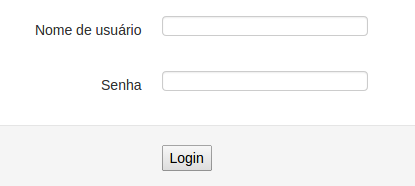
\includegraphics[scale=0.6]{images/entrada.png}
     \caption{Entrada no sistema}
     \label{fig:entrada}
\end{figure}

    Entre com o usuário padrão "administrator" e a senha "icpedu". Será mostrado uma tela para cadastro do novo administrador do sistema, como mostra a figura \ref{fig:inicioadmin}.

\begin{figure}[ht]
     \centering
     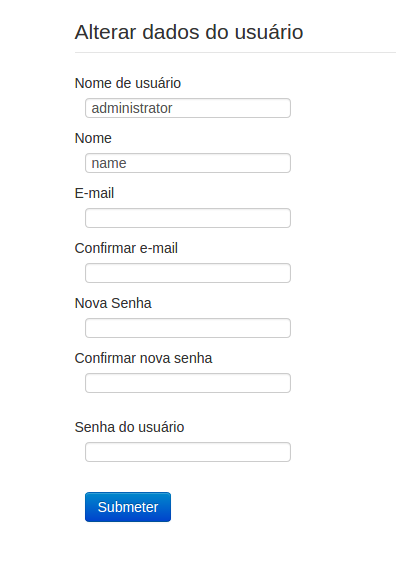
\includegraphics[scale=0.5]{images/inicioadmin.png}
     \caption{Cadastro do administrador}
     \label{fig:inicioadmin}
\end{figure}

    Preencha os campos com a informação exigida, sem deixar nada em branco. 
    
    Grave bem o "Nome de usuário" e a "Nova senha", pois a partir de agora estas serão as credenciais exigidas, tanto nas próximas etapas de configuração, quanto nas próximas vezes que desejar entrar no sistema. Em "senha do usuário", insira a senha do administrador anterior "icpedu" para confirmar a operação. Você será redirecionado para a etapa de backup, como mostra a figura \ref{fig:opcaobackup}.
    
    \begin{figure}[ht]
     \centering
     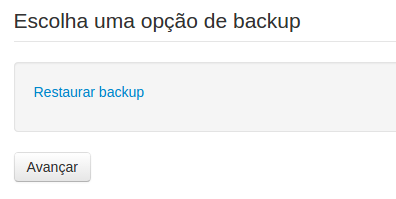
\includegraphics[scale=0.6]{images/opcaobackup.png}
     \caption{Opção de backup}
     \label{fig:opcaobackup}
\end{figure}

    Se existir algum backup do sistema, é possível recuperá-lo nesse passo, clicando em \textit{Restaurar backup} e fazendo upload do arquivo de backup gerado anteriormente. Se não houver backup, ignore esta etapa e clique em \textit{Avançar}. 
    
    Em seguida é necessário escolher uma opção para armazenamento da chave da Autoridade Certificadora. A seguinte tela será mostrada:
    
    \begin{figure}[ht]
     \centering
     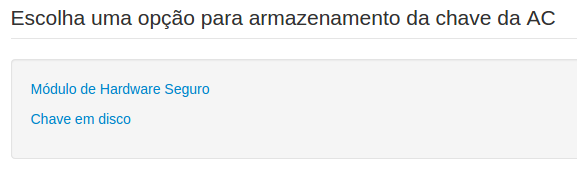
\includegraphics[scale=0.6]{images/armazenachave.png}
     \caption{Opção de armazenamento de chave}
     \label{fig:armazenachave}
\end{figure}

    Se for escolhida a opção "Chave em disco", será solicitada a criação de uma requisição a ser aceita por uma Autoridade Certificadora. Para exemplo, neste manual usaremos a opção "Módulo de Hardware Seguro". Ao optar por esse modo de armazenamento, o usuário será redirecionado para a página de registro e configuração do Módulo de Hardware Seguro, como mostra a figura \ref{fig:confighsm}.
    
    É possível selecionar uma engine já existente no sistema, através da opção \textit{Engine $>$ Selecionar arquivo existente}, ou enviar a sua própria engine, através da opção \textit{Engine $>$ Enviar arquivo}. Independente da escolha, é necessário informar o ID da engine e o identificador da chave do MSC.
    
    Na parte dos comandos, insira o IP e a porta específica de comunicação com o Módulo de Hardware Seguro. Insira sua senha de administrador, escolhida na primeira etapa do cadastro, e clique em \textit{Submeter}.
    
    \begin{figure}[ht]
     \centering
     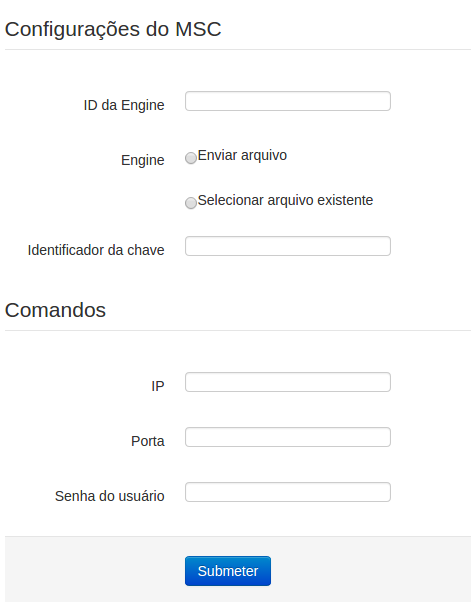
\includegraphics[scale=0.5]{images/confighsm.png}
     \caption{Configuração do MSC}
     \label{fig:confighsm}
\end{figure}

    Depois de configurá-lo, você será redirecionado para a página de criação de requisição para o seu sistema de emissão de certificados ICPEdu. Esta requisição deve ser aprovada por uma Autoridade Certificadora superior, que irá gerar um certificado para o sistema. 

    Preencha os campos da requisição com os dados solicitados sobre sua organização e clique em \textit{Submeter}. Você será redirecionado para a seguinte tela:
    
    \begin{figure}[ht]
     \centering
     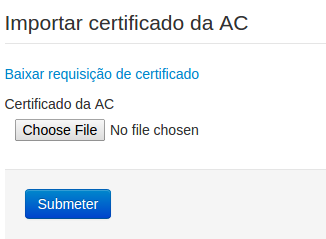
\includegraphics[scale=0.6]{images/importacertAC.png}
     \caption{Importação de certificado}
     \label{fig:reqcert}
\end{figure}

    Baixe a requisição gerada e a envie para uma Autoridade Certificadora, solicitando que esta seja aprovada. Quando isto ocorrer, um certificado será gerado. Faça o download do certificado do seu sistema e importe ele, como mostra a figura \ref{fig:reqcert}.
    
    Em seguida você será redirecionado para a seguinte tela:
    
    \begin{figure}[ht]
     \centering
     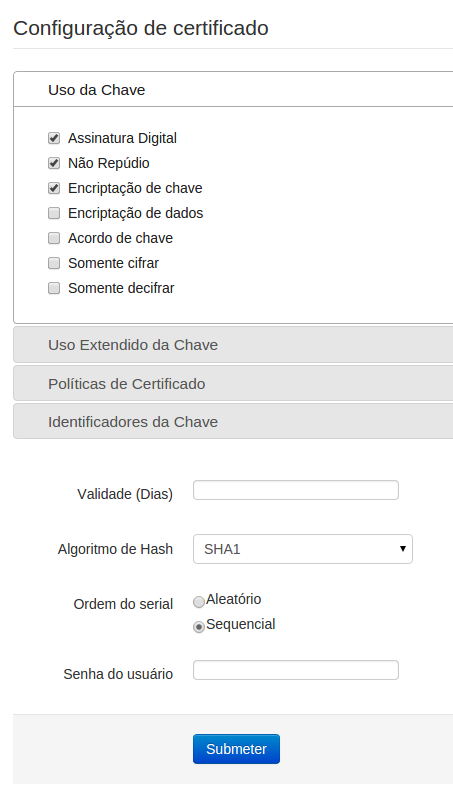
\includegraphics[scale=0.5]{images/configcertificado.png}
     \caption{Configuração do certificado}
     \label{fig:configcertificado}
\end{figure}

    Nesta etapa é possível configurar seu certificado. Algumas opções são definidas por padrão, mas você pode mudá-las se assim desejar. O mesmo serve para o algoritmo de hash e a ordem do serial do certificado. É obrigatório fornecer a validade do seu certificado em dias. Por fim, insira sua senha de administrador e clique em \textit{Submeter}.
    
    Ao fazer isso, você será redirecionado para a página de configuração de whitelist. Whitelist é uma lista com os IPs das máquinas que estão autorizadas a emitir certificado. Quem gerencia esta lista para cada organização são os respectivos operadores das mesmas. O administrador pode escolher se deseja ou não trabalhar com o sistema de whitelist. Faça sua escolha e clique em \textit{Submeter}.
    
    A próxima etapa da configuração é selecionar a federação a qual o seu sistema pertence. É possível selecionar a Comunidade Acadêmica Federada (CAFe) ou a Chimarrão. Pode-se ainda escolher outra federação não listada, e neste caso deve-se fornecer as URLs da mesma.
    
    Depois de selecionar a federação, você será redirecionado para a última etapa da configuração, que é destinada ao registro do primeiro operador do sistema, como é mostrado na figura a seguir:
    
    \begin{figure}[ht]
     \centering
     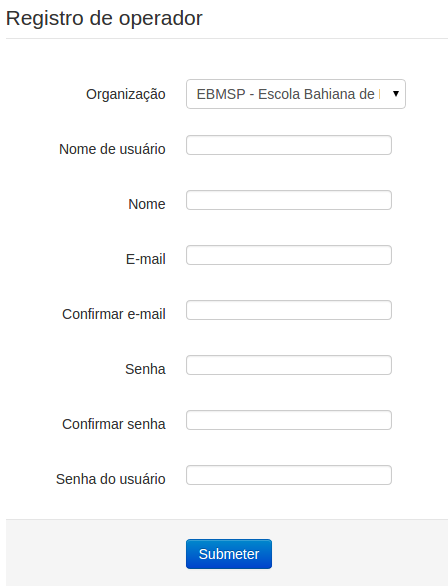
\includegraphics[scale=0.5]{images/inicioregistroop.png}
     \caption{Registro de operador}
     \label{fig:inicioregop}
\end{figure}

    Preencha os dados do operador conforme são solicitados e clique em \textit{Submeter}. Ao fazer isto, a configuração será concluída e você será redirecionado para a página inicial do sistema de emissão de certificados ICPEdu, onde verá o menu funcional do sistema (a ser explicado nos próximos capítulos) e as tarefas pendentes, como mostra a figura a seguir:
    
    \begin{figure}[ht]
     \centering
     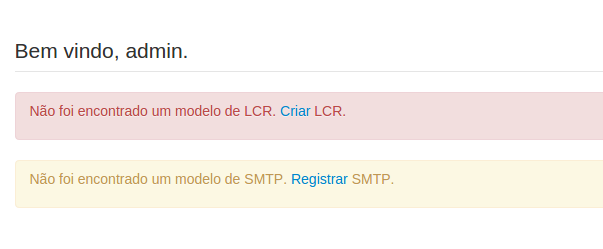
\includegraphics[scale=0.5]{images/pendencias.png}
     \caption{Tarefas pendentes}
     \label{fig:pendencias}
\end{figure}

%\chapter{Perfil Administrador}\label{cap:criador}
%% !Mode:: "TeX:UTF-8"

Neste capítulo serão apresentadas as funcionalidades disponíveis ao administrador após a instalação do sistema, referentes ao registro de operadores e gerenciamento das funções disponíveis no sistema.

A parte do administrador é destinada à criação de operadores, cadastro de MSCs e configuração dos modelos de LCR e certificado, bem como à gerência dos certificados emitidos e revogados e suas respectivas estatísticas por tempo e organização. O administrador é também o responsável por exportar e conferir os logs do sistema.

Ao logar como administrador é possível visualizar as tarefas pendentes.

\section{Operadores}\label{sec:operadores}

Ao logar-se como administrador, é possível ver o menu de funções. Ao clicar em \textit{Operadores}, duas possibilidades serão mostradas: \textit{Listar} e \textit{Registrar}.


\subsection{Registrar operadores}\label{subsec:cadEntidades}

Os passos para registrar um operador são simples. Basta selecionar a opção \textit{Registrar} no menu \textit{Operador}. Será carregada uma página, como mostra a figura \ref{fig:registroop}.

\begin{figure}[ht]
     \centering
     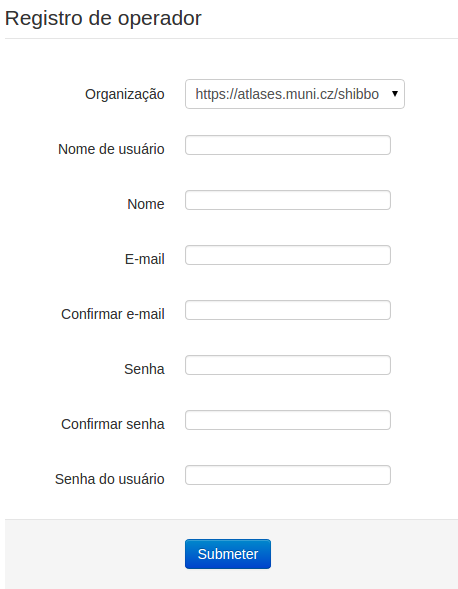
\includegraphics[scale=0.6]{images/registroop.png}
     \caption{Registro de Operador}
     \label{fig:registroop}
\end{figure}

Os campos abaixo devem ser preenchidos com os dados do Operador que está sendo cadastrado:

\begin{itemize}

	\item \textbf{Organização:} Selecione a organização a qual o operador está afiliado;
	\item \textbf{Nome de usuário:} Preencha o nome que o operador deverá utilizar para logar no sistema;
	\item \textbf{Nome:} Preencha o nome completo do operador;
	\item \textbf{E-mail:} Preencha este campo com o respectivo e-mail do operador e repita-o no campo seguinte;
	\item \textbf{Senha:} Escolha uma senha que o operador deverá utilizar para logar no sistema e confirme-a no campo seguinte;
	\item \textbf{Senha do usuário:} Insira a sua senha de administrador para confirmar a operação.
	
\end{itemize}

\subsection{Listar Operadores}

No menu \textit{Operadores $>$ Listar}, o usuário é capaz de visualizar os operadores já cadastrados.
Na página aparecerá uma lista com todos os operadores, semelhante à imagem \ref{fig:listarop}.
Na aba onde são listados é possível ver \textit{Nome de usuário, Nome, Email, Organização e Ação} de cada operador registrado. As ações possíveis são:

\begin{itemize}

	\item \textbf{Excluir operador(}\begin{wrapfigure} 
\includegraphics[height=10]{images/iconedelete2} \end{wrapfigure} \textbf{):} Remove o operador do banco. O mesmo não poderá mais logar no sistema.
	\item \textbf{Editar operador(}\begin{wrapfigure} 
\includegraphics[height=10]{images/iconeeditar} \end{wrapfigure} \textbf{):} É mostrada uma tela onde é possível alterar alguns dados do operador.
	
\end{itemize}

\begin{figure}[ht]
     \centering
     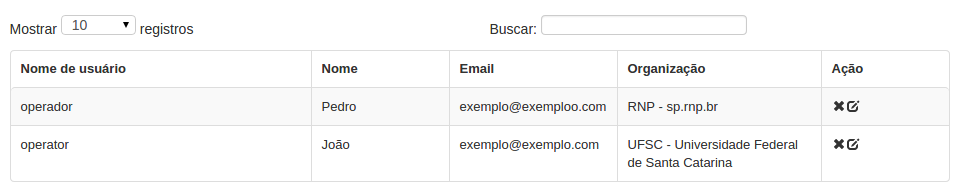
\includegraphics[scale=0.5]{images/listarop.png}
     \caption{Listagem de Operadores}
     \label{fig:listarop}
\end{figure}

\section{SMTP}

\subsection{Registrar SMTP}

SMTP(do inglês \textit{Simple Mail Transfer Protocol}) é o protocolo padrão para envio de e-mails através da Internet. É necessário configurar o e-mail e as mensagens automáticas que devem ser enviadas para o mesmo caso ocorra algum erro ou algum certificado seja emitido.
Para registrar o SMTP deve-se ir ao ícone \textit{SMTP $>$ Registrar}. Será carregada uma página, como mostra a figura \ref{fig:smtp}. É escolha do administrador utilizar uma autenticação extra ou cadastrar sem autenticação (quando não é preciso inserir login e senha do e-mail). 

Caso escolha registrar sem autenticação, siga estes passos:

\begin{itemize}
	\item \textbf{Host Smtp} : Utilizar o IP do servidor SMTP do seu e-mail;
	\item \textbf{E-mail}: E-mail para qual as mensagens devem ser enviadas;
	\item \textbf{Porta}: Se este campo for deixado em branco, será utilizada a porta padrão para as configurações fornecidas. Forçar a utilização de alguma outra porta pode dar problema, por isso forneça uma porta somente se tiver certeza que esta pode ser utilizada com as configurações fornecidas;
    \item \textbf{Tipo de autenticação}: Selecione \textit{Sem autenticação}. Marque a caixa para \textit{Mandar um e-mail teste}. Você deve receber a confirmação do registro de SMTP no e-mail fornecido;
    \item \textbf{Senha do usuário}: Senha do administrador.
\end{itemize}

Caso escolha utilizar algum tipo de autenticação, siga estes passos:

\begin{itemize}
	\item \textbf{Host Smtp} : Utilizar o caminho para o SMTP do seu e-mail. Por exemplo, o caminho para um e-mail do \textit{gmail} seria \textit{smtp.gmail.com};
	\item \textbf{E-mail}: E-mail para qual as mensagens devem ser enviadas;
	\item \textbf{Porta}: Se este campo for deixado em branco, será utilizada a porta padrão para as configurações fornecidas. Forçar a utilização de alguma outra porta pode dar problema, por isso forneça uma porta somente se tiver certeza que esta pode ser utilizada com as configurações fornecidas;
    \item \textbf{Tipo de autenticação}: Selecione \textit{Usuário e Senha}, \textit{Plain} ou \textit{CramMD5}. Marque a caixa para \textit{Mandar um e-mail teste}. Você deve receber a confirmação do registro de SMTP no e-mail fornecido;
    \item \textbf{Protocolo criptográfico}: Selecione \textit{Nenhum}, \textit{SSL} ou \textit{TLS}. Note que alguns servidores de e-mail não aceitam a opção \textit{Nenhum};
    \item \textbf{Nome de usuário}: Informe o login utilizado para entrar no e-mail fornecido;
    \item \textbf{Senha}: Informe a senha utilizada para entrar no e-mail fornecido e confirme-a no campo seguinte;
    \item \textbf{Senha do usuário}: Insira a sua senha de administrador para confirmar a operação.
\end{itemize}

\begin{figure}[ht]
     \centering
     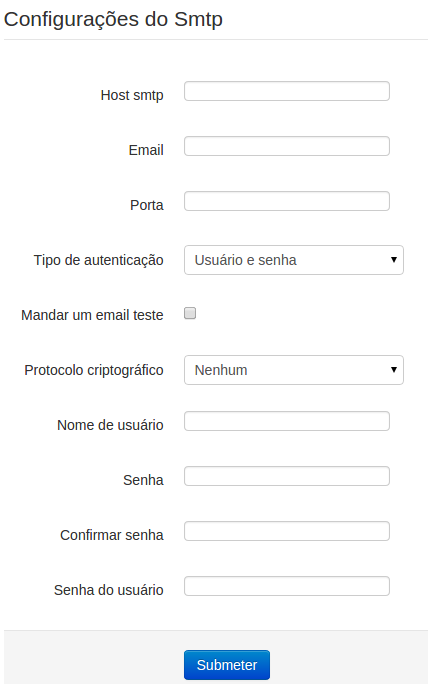
\includegraphics[scale=0.6]{images/smtp.png}
     \caption{Registrar SMTP}
     \label{fig:smtp}
\end{figure}

\subsection{Configurar Mensagens}

Nesta parte do sistema o administrador pode configurar as mensagens que serão enviadas para o seu e-mail de forma automática quando algum evento acontecer. Para configurar as mensagens do SMTP deve-se ir ao ícone \textit{SMTP $>$ Configurar mensagens}. Será carregada uma página, como mostra a figura \ref{fig:msgsmtp}. É possível configurar o assunto e o conteúdo do e-mail para os seguintes eventos:

\begin{itemize}
	\item \textbf{E-mail teste}: É enviado quando um SMTP é registrado com sucesso;
	\item \textbf{Certificado emitido}: É enviado quando um certificado é emitido com sucesso;
	\item \textbf{Erro ao emitir certificado - Sem operadores registrados}: É enviado quando um certificado não pôde ser emitido porque não há nenhum operador registrado no sistema;
	\item \textbf{Erro ao emitir certificado}: É enviado quando ocorre um erro na emissão do certificado;
	\item \textbf{Erro na emissão automática de LCR}: Como será mostrado posteriormente neste manual, é possível configurar a periodicidade em que uma LCR(\textit{Lista de Certificados Revogados}) será emitida. Este tipo de e-mail é enviado quando ocorre um erro nesta emissão automática de LCRs;
	\item \textbf{Erro ao emitir um certificado - Instituição não cadastrada}: É enviado quando um certificado não pôde ser emitido porque não há um operador registrado para a organização que tentou emitir o certificado.
\end{itemize}

\begin{figure}[ht]
     \centering
     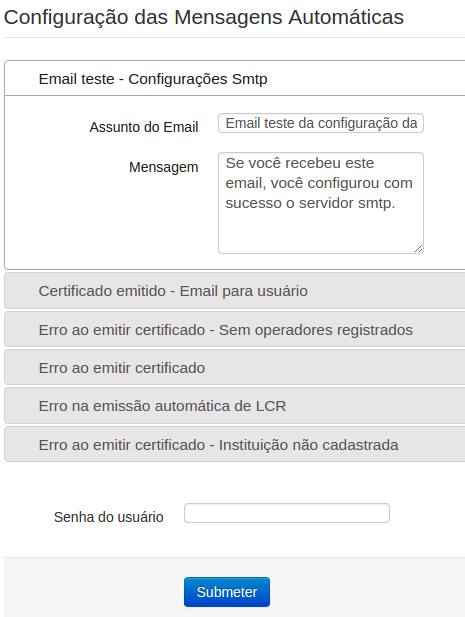
\includegraphics[scale=0.6]{images/msgsmtp.png}
     \caption{Configurar Mensagens}
     \label{fig:msgsmtp}
\end{figure}

\section{Modelos}

Esta é a parte onde deve-se configurar o modelo das LCRs e dos Certificados que serão emitidos.

\subsection{LCR}

Para configurar o template de LCR, basta selecionar o menu \textit{Modelos $>$ LCR}. Aparecerá uma tela igual à imagem \ref{fig:modelolcr} mostrada abaixo. O usuário deve marcar a caixa "Emissão automática" se quiser que a LCR seja emitida de forma automática. Caso não selecione esta opção, deve prosseguir escolhendo logo a baixo a validade da LCR que será emitida, lembrando que só é possível usar uma validade menor que um ano. Deve escolher também o algoritmo que assina a LCR.
Por último deve-se digitar a senha do administrador e clicar no botão \emph{Submeter}.

\begin{figure}[ht]
     \centering
     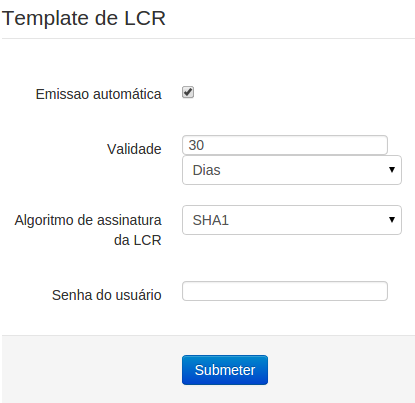
\includegraphics[scale=0.5]{images/modelolcr.png}
     \caption{Modelo de LCR}
     \label{fig:modelolcr}
\end{figure}

\subsection{Certificado}

O administrador deve clicar em \textit{Modelos $>$ Certificado}. Será mostrada uma tela como na figura \ref{fig:modelocert}. É possível configurar vários aspectos do certificado:

\begin{itemize}
	\item \textbf{Uso da chave}: Algumas opções já vêm marcadas por default, mas o administrador pode desmarcá-las se assim desejar. Marque/desmarque o que for desejado e prossiga para a próxima etapa da configuração;
	\item \textbf{Uso extendido da chave}: Nesta etapa, as duas opções disponíveis vêm marcadas por default. Desmarque se for necessário, ou prossiga para a próxima etapa;
	\item \textbf{Políticas de certificado}: Insira os identificadores da Política do Certificado e da Declaração de Práticas de Certificação, se existir;
	\item \textbf{Identificadores da chave}: Os dois identificadores da chave estão marcados por default. Desmarque se for necessário, ou prossiga para a próxima etapa;
	\item \textbf{Validade}: Informe a validade do certificado em dias. Lembrando que esta deve ser um número inteiro de 1 a 3650;
	\item \textbf{Algoritmo de Hash}: Escolha algoritmo que vai assinar o certificado;
	\item \textbf{Odem do serial}: Escolha se deseja que a ordem seja sequencial ou aleatória;
	\item \textbf{Senha do usuário}: Informe a senha do administrador e clique no botão \emph{Submeter}.
\end{itemize}

\begin{figure}[ht]
     \centering
     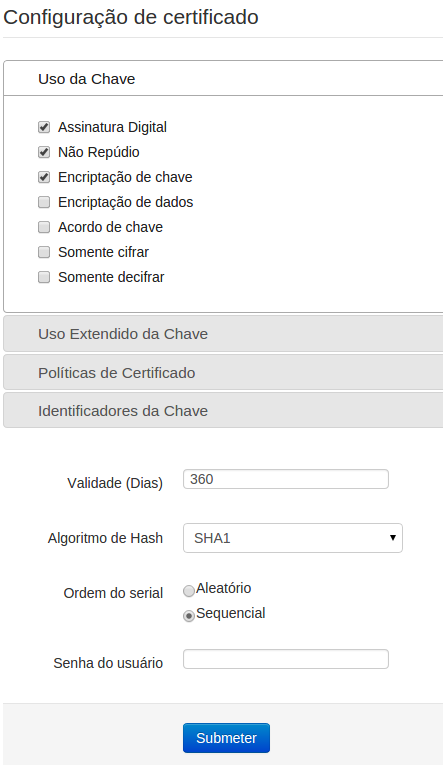
\includegraphics[scale=0.5]{images/modelocert.png}
     \caption{Modelo de Certificado}
     \label{fig:modelocert}
\end{figure}

\section{LCR}

Esta é a parte do sistema que permite que o administrador emita uma Lista de Certificados Revogados até o momento e faça o Download da LCR que desejar.

\subsection{Emitir}

Para emitir uma LCR é preciso acessar o menu \textit{LCR $>$ Emitir}. Basta informar a senha de administrador e clicar \emph{Submeter}. O sistema vai emitir uma lista com todos os certificados revogados até o momento.

\subsection{Download}

Para fazer o download de uma LCR é preciso acessar o menu \textit{LCR $>$ Download}. É possível fazer download de duas formas diferentes, como mostra a figura \ref{fig:lcr}. Se desejar ver as LCRs emitidas em um período específico de tempo, escolha a data de início e fim e clique no botão \emph{Ver LCRs}. Caso deseje ver apenas a última LCR emitida, deixa os campos de início e fim vazios e clique no botão \emph{Baixar a última LCR}.

\begin{figure}[ht]
     \centering
     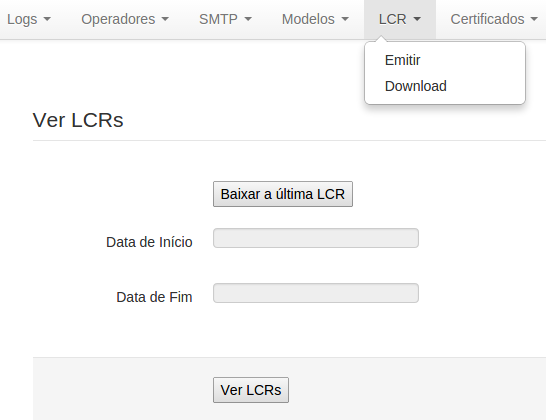
\includegraphics[scale=0.6]{images/lcr.png}
     \caption{Download de LCR}
     \label{fig:lcr}
\end{figure}

\section{Certificados}

No menu \textit{Certificados} é possível listar todos os certificados emitidos até o momento, estejam eles ativos ou revogados. Acesse o menu \textit{Certificados $>$ Listar}. Aparecerá uma tela como mostra a figura \ref{fig:listarcert}. Nesta página é possível ver a organização e o e-mail do operador afiliado à organização responsável pela emissão do certificado, a data em que foi emitido e a data em que este irá expirar e o estado em que se encontra (Ativo ou revogado).
É possível realizar as seguintes ações:

\begin{itemize}

	\item \textbf{Download do certificado(}\begin{wrapfigure} 
\includegraphics[height=10]{images/iconedownload} \end{wrapfigure} \textbf{):} Ao clicar nesse ícone você faz o download do certificado selecionado.
	\item \textbf{Revogar certificado(}\begin{wrapfigure} 
\includegraphics[height=10]{images/iconedelete2} \end{wrapfigure} \textbf{):} Quando um certificado estiver ativo, este ícone irá aparecer na linha do respectivo certificado para que este possa ser revogado individualmente. Se houver necessidade de revogar mais certificados, é possível selecioná-los e revogalos de uma só vez através do ícone de revogação no canto inferior direito da imagem. 
	
\end{itemize}

\begin{figure}[ht]
     \centering
     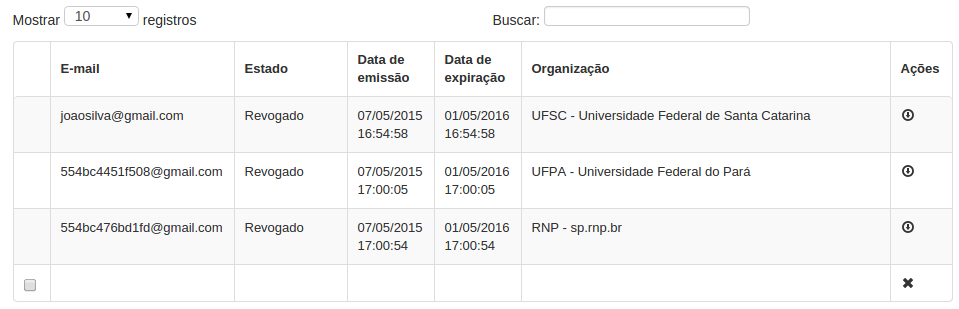
\includegraphics[scale=0.5]{images/listarcert.png}
     \caption{Listagem de certificados}
     \label{fig:listarcert}
\end{figure}

\section{Backup}

Fazer um backup do sistema significa salvar toda a sua estrutura. O backup contém todas as operações realizadas até o momento. O backup do sistema de emissão de certificados ICPEdu é cifrado, pelo fato de poder haver dados sigilosos, a partir de uma senha que será escolhida pelo usuário.

\subsection{Gerar}

Para gerar o backup, basta selecionar o menu \textit{Backup $>$ Gerar}. Aparecerá uma tela igual à imagem \ref{fig:gerarbackup} mostrada abaixo. O usuário deve preencher o primeiro campo com a senha para cifrar o backup e confirmá-la no campo abaixo. É importante armazenar essa senha em local seguro, pois sem ela, será impossível restaurar o backup.
Por último deve-se digitar a senha do usuário e clicar no botão \emph{Submeter}.

\begin{figure}[ht]
     \centering
     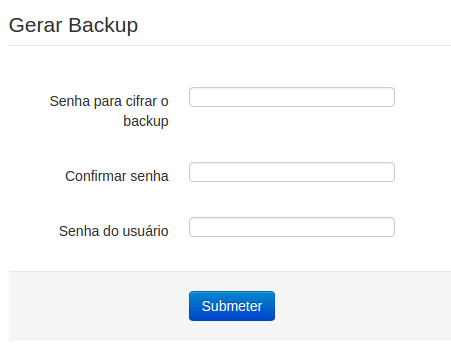
\includegraphics[scale=0.6]{images/gerarbackup.png}
     \caption{Gerar Backup}
     \label{fig:gerarbackup}
\end{figure}

\subsection{Restaurar}

O administrador deve entrar no sistema e clicar em \textit{Backup $>$ Restaurar}. Será mostrada a seguinte tela \ref{fig:restaurarbackup}:

\begin{figure}[ht]
     \centering
     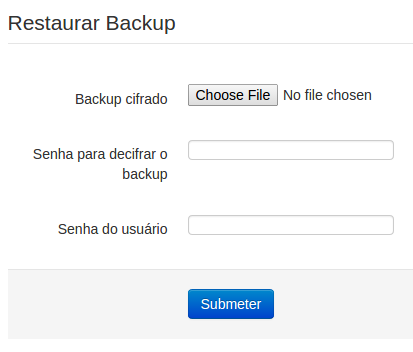
\includegraphics[scale=0.6]{images/restaurarbackup.png}
     \caption{Restaurar Backup}
     \label{fig:restaurarbackup}
\end{figure}

No primeiro campo o usuário deve selecionar o arquivo de backup, gerado e salvo na etapa anterior. Depois deve digitar a senha para decifrar o backup, que deve ser a mesma definida na etapa de geração de backup. Por último, informe a senha do administrador e clique no botão \textit{Submeter}.

\section{Estatísticas}

Esta parte do sistema destina-se à mostrar as estatísticas (por tempo ou por organização) dos certificados emitidos. É possível verificar quantos certificados já foram emitidos e quantos ainda estão ativos. Quando já houver muitos certificados emitidos no sistema, é mais rápido e prático consultar as estatísticas do que contar a quantidade de certificados listados no menu \textit{Certificados}.

\subsection{Total}

Acesse o menu \textit{Estatísticas $>$ Total}. Aparecerá uma tela como mostra a figura \ref{fig:estotal}. É possível ver quantos certificados já foram emitidos no total, bem como quantos ainda estão ativos, quantos já foram revogados e quantos estão expirados. Logo em baixo é possível clicar nas organizações e ver as estatísticas em separado de cada uma delas. Lembrando que, para poder ver a estatística de uma organização específica, é necessário possuir um operador cadastrado para ela, do contrário a organização não aparecerá na tela como mostrado na figura abaixo.

\begin{figure}[ht]
     \centering
     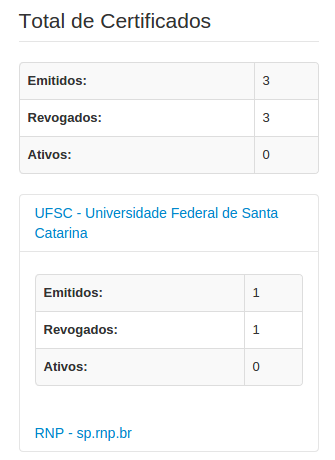
\includegraphics[scale=0.6]{images/estatisticatotal.png}
     \caption{Estatísticas total}
     \label{fig:estotal}
\end{figure}

\subsection{Procurar por tempo}

Acesse o menu \textit{Estatísticas $>$ Procurar por tempo}. Aparecerá uma tela como mostra a figura \ref{fig:estempo}.

\begin{figure}[ht]
     \centering
     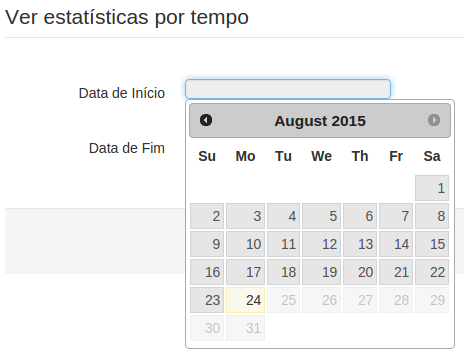
\includegraphics[scale=0.5]{images/estatisticatempo.png}
     \caption{Estatísticas por tempo}
     \label{fig:estempo}
\end{figure}

Para ver a estatística dos certificados emitidos em um período específico de tempo, escolha a data de início e fim e clique no botão \emph{Ver Estatísticas}.

\section{Atributos}

Através do menu \textit{Atributos $>$ Mapeador de atributos} o administrador pode escolher quais atributos o certificado vai requerer, como mostra a figura \ref{fig:atmap}.

\begin{figure}[ht]
     \centering
     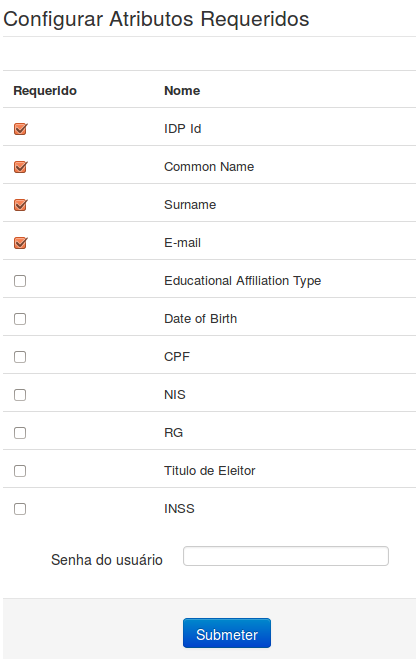
\includegraphics[scale=0.6]{images/attributesmapper.png}
     \caption{Mapeador de atributos}
     \label{fig:atmap}
\end{figure}

Marque os atributos que devem aparecer obrigatoriamente no seu certificado, insira sua senha de administrador e clique no botão \textit{Submeter}.

\section{Cron}

Através do menu \textit{Cron $>$ Tarefas do Cron} é possível verificar as próximas tarefas agendadas para o Cron e também agendar uma nova.

\subsection{Emissão automática de LCR}

Caso o administrador já tenha configurado a periodicidade em que as LCRs devem ser emitidas (pode ser feito através do menu \textit{Modelos $>$ LCR}), será possível verificar sua próxima emissão, sem ser possível alterá-la, como mostra a figura \ref{fig:cron}.

\begin{figure}[ht]
     \centering
     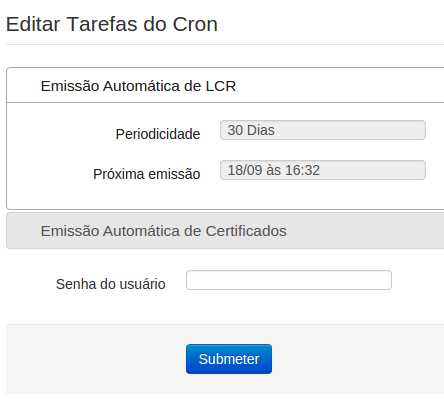
\includegraphics[scale=0.5]{images/cron.png}
     \caption{Emissão automática de LCR}
     \label{fig:cron}
\end{figure}

\subsection{Emissão automática de Certificados}

É possível editar as tarefas do Cron que tratam da parte de certificados. Para fazer isso, basta assinar a caixa \textit{Agendar} e inserir a periodicidade desejada, como mostra a figura \ref{fig:croncert}.

\begin{figure}[ht]
     \centering
     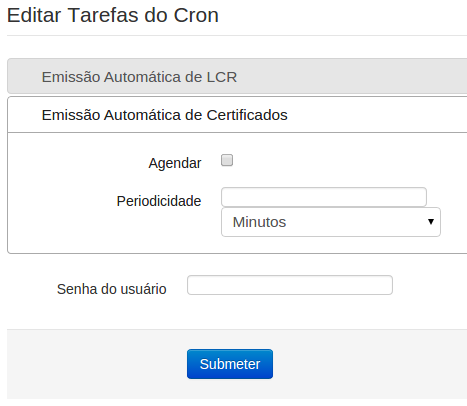
\includegraphics[scale=0.5]{images/croncert.png}
     \caption{Emissão automática de Certificados}
     \label{fig:croncert}
\end{figure}

Insira sua senha de administrador e clique no botão \textit{Submeter}.

\section{Alterar dados do usuário e Sair}

O administrador poder alterar seus dados pessoais e sair do sistema a qualquer momento, basta clicar na engrenagem localizada ao lado superior direito da tela. Duas operações aparecerão: \textit{Alterar dados do usuário} e \textit{Sair}. Ao clicar em \textit{Alterar dados do usuário}, aparecerá uma tela com os campos de dados pessoais, como mostra a figura \ref{fig:alteraadmin}. Altere o que desejar, insira a sua senha de administrador e clique no botão \emph{Submeter}.

\begin{figure}[ht]
    \centering
     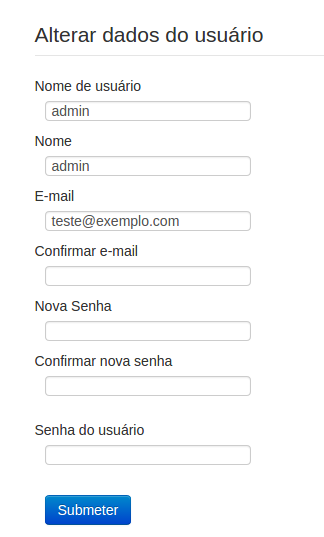
\includegraphics[scale=0.5]{images/alterardadosadmin.png}
     \caption{Alterar dados do usuário}
     \label{fig:alteraadmin}
\end{figure}

\section{Logs}\label{sec:logs}

O administrador pode exportar ou apagar os \textit{logs} do sistema a qualquer momento. Este arquivo contém todas as operações efetuadas pelo sistema de emissão de certificados ICPEdu até o momento em que o \textit{log} tenha sido exportado, em um formato de texto, onde cada ação é uma frase. Para fazer qualquer uma das duas operações, vá ao menu \textit{Logs}, como mostra a figura \ref{fig:logs}.

\begin{figure}[ht]
    \centering
     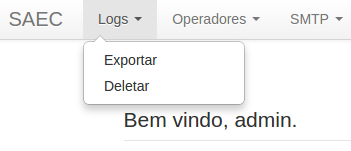
\includegraphics[scale=0.5]{images/logs.png}
     \caption{Menu Logs}
     \label{fig:logs}
\end{figure}

\subsection{Deletar Logs}

Para apagar seus \textit{logs}, basta clicar no menu \textit{Logs $>$ Deletar}. O administrador será direcionado para uma tela que pedirá sua senha para confirmar a ação. 

\subsection{Exportar Logs}

No menu \textit{Logs $>$ Exportar}, pode-se exportar os \textit{logs} do usuário. Ao clicar, o download acontecerá automaticamente. Abra o arquivo e verifique as últimas ações. Caso o \textit{log} tenha sido deletado anteriormente, esta ação deverá estar presente no arquivo.

 

%\chapter{Perfil Operador}\label{cap:oper-ar}
%                  
% !Mode:: "TeX:UTF-8"

Neste capítulo serão apresentadas as funcionalidades disponíveis aos operadores após a instalação do sistema e cadastro dos mesmos.
A parte do operador é destinada à listagem dos certificados emitidos para sua organização. É possível ver as estatísticas destes certificados e mapear os atributos dos mesmos corretamente.

\section{Certificados}

No menu \textit{Certificados} é possível listar todos os certificados emitidos até o momento para a organização na qual o operador está afiliado, estejam eles ativos ou revogados. Acesse o menu \textit{Certificados $>$ Listar}. Aparecerá uma tela como mostra a figura \ref{fig:listarcertop}. Nesta página é possível ver a data em que foi emitido e a data em que irá expirar cada certificado e o estado em que se encontra (Ativo ou revogado).
É possível realizar as seguintes ações:

\begin{itemize}

	\item \textbf{Download do certificado(}\begin{wrapfigure} 
\includegraphics[height=10]{images/iconedownload} \end{wrapfigure} \textbf{):} Ao clicar nesse ícone você faz o download do certificado selecionado.
	\item \textbf{Revogar certificado(}\begin{wrapfigure} 
\includegraphics[height=10]{images/iconedelete2} \end{wrapfigure} \textbf{):} Quando um certificado estiver ativo, este ícone irá aparecer na linha do respectivo certificado para que este possa ser revogado individualmente. Se houver necessidade de revogar mais certificados, é possível selecioná-los e revogalos de uma só vez através do ícone de revogação no canto inferior direito da imagem. 
	
\end{itemize}

\begin{figure}[ht]
     \centering
     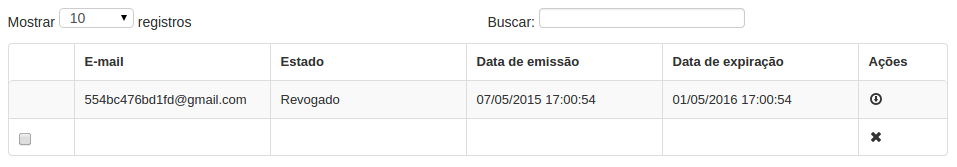
\includegraphics[scale=0.5]{images/listarcertop.png}
     \caption{Listagem de certificados}
     \label{fig:listarcertop}
\end{figure}

\section{Estatísticas}

Esta parte do sistema destina-se à mostrar as estatísticas dos certificados emitidos. É possível verificar quantos certificados já foram emitidos e quantos ainda estão ativos.

\subsection{Total}

Acesse o menu \textit{Estatísticas $>$ Total}. Aparecerá uma tela como mostra a figura \ref{fig:estotalop}. É possível ver quantos certificados já foram emitidos no total, bem como quantos ainda estão ativos, quantos já foram revogados e quantos estão expirados. Lembrando que, diferentemente do perfil de administrador, que pode ver as estatísticas por organização, neste perfil o operador verá apenas a estatística que diz respeito à organização na qual está afiliado.

\begin{figure}[ht]
     \centering
     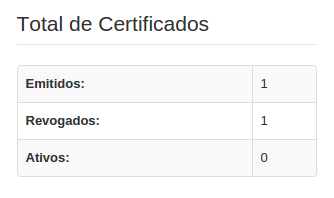
\includegraphics[scale=0.6]{images/estatisticaop.png}
     \caption{Estatísticas total}
     \label{fig:estotalop}
\end{figure}

\subsection{Procurar por tempo}

Acesse o menu \textit{Estatísticas $>$ Procurar por tempo}. Aparecerá uma tela como mostra a figura \ref{fig:estempo}.

\begin{figure}[ht]
     \centering
     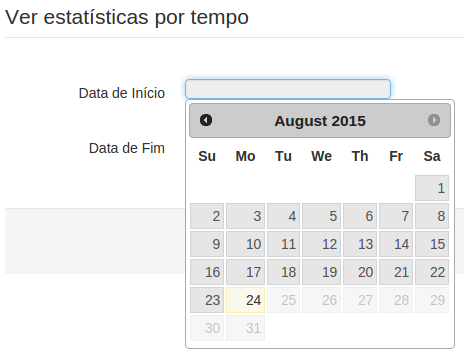
\includegraphics[scale=0.5]{images/estatisticatempo.png}
     \caption{Estatísticas por tempo}
     \label{fig:estempo}
\end{figure}

Para ver a estatística dos certificados emitidos em um período específico de tempo, escolha a data de início e fim e clique no botão \emph{Ver Estatísticas}.

\section{Atributos}

Através do menu \textit{Atributos $>$ Mapeador de atributos} o operador pode configurar os dados que vêm da federação e que vão pertencer ao certificado, como mostra a figura \ref{fig:atmapop}.

\begin{figure}[ht]
     \centering
     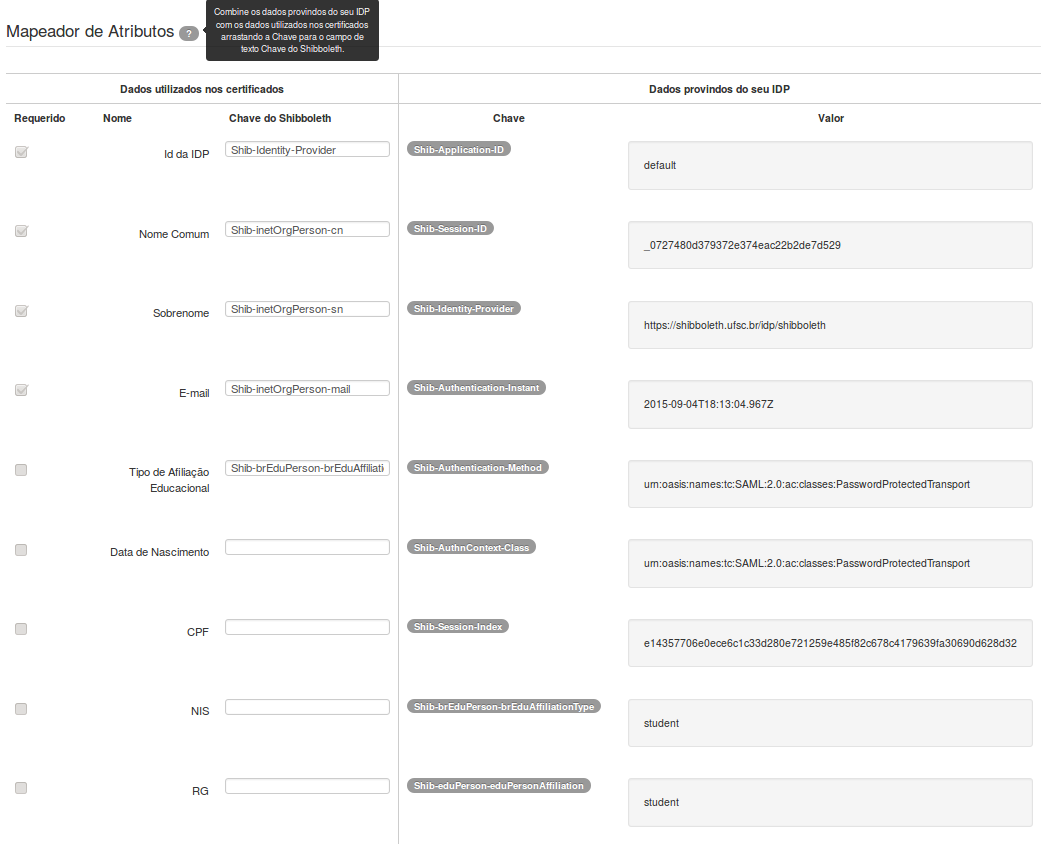
\includegraphics[scale=0.4]{images/oper_attributesmapper.png}
     \caption{Mapeador de atributos}
     \label{fig:atmapop}
\end{figure}

Quando o operador acessar esta tela, os atributos que são necessários configurar já vão vir marcados, pois é o administrador que determina quais atributos vão aparecer no certificado. A tarefa do operador é verificar cada dado que vem da federação e colocá-lo no campo adequado. Por exemplo: Se o CPF for um atributo obrigatório, selecione o CPF na coluna direita, onde estão os dados da federação, e arraste-o para o respectivo campo de CPF na coluna esquerda, onde estão os dados do certificado. Qualquer dúvida que o operador tenha, basta passar o mouse por cima do ponto de interrogação no lado superior esquerdo da tela e encontrará explicação da tarefa. 

\section{Alterar dados do usuário e Sair}

O operador poder alterar seus dados pessoais e sair do sistema a qualquer momento, basta clicar na engrenagem localizada ao lado superior direito da tela. Duas operações aparecerão: \textit{Alterar dados do usuário} e \textit{Sair}. Ao clicar em \textit{Alterar dados do usuário}, aparecerá uma tela com os campos de dados pessoais, como mostra a figura \ref{fig:alterarop}. Altere o que desejar, lembrando que não é possível alterar sua organização. Insira a sua senha e clique no botão \emph{Submeter}. Ao clicar em \textit{Sair}, o usuário sai do sistema.

\begin{figure}[ht]
    \centering
     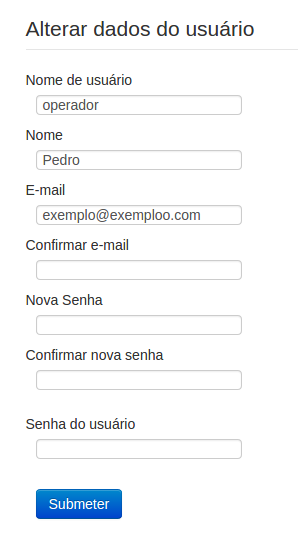
\includegraphics[scale=0.7]{images/alterardadosop.png}
     \caption{Alterar dados do usuário}
     \label{fig:alterarop}
\end{figure} 

\chapter{Usuário final}\label{cap:ufinal-ar}
Neste capítulo serão apresentadas as funcionalidades disponíveis aos usuários finais do sistema.
 É possível emitir, visualizar, exportar e revogar um certificado digital, bem como acessar as páginas de ajuda e de repositório do sistema.

\section{Emissão de Certificado}

No menu \textit{Certificado} é possível encontrar as ações de emitir e revogar, como mostra a figura \ref{fig:emirevog}:

\begin{figure}[ht]
     \centering
     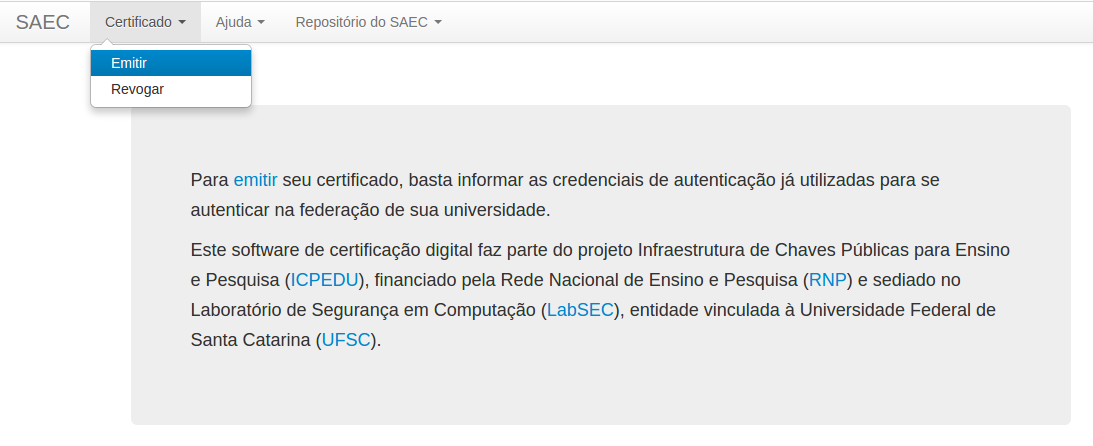
\includegraphics[scale=0.4]{images/emitir1.png}
     \caption{Tela inicial}
     \label{fig:emirevog}
\end{figure}

Para emitir, é necessário selecionar a instituição na qual você é afiliado. Seguiremos o manual utilizando a Universidade Federal de Santa Catarina (UFSC) como exemplo de instituição provedora de identidade. Ao ser redirecionado para a tela de escolha de Federação, selecione sua instituição. Você será redirecionado para a página de autenticação da sua instituição, onde deve entrar com os dados do seu usuário já cadastrado. Os passos descritos aqui podem ser observados nas figuras \ref{fig:ufxc} e \ref{fig:ufxc2}.

\begin{figure}[ht]
     \centering
     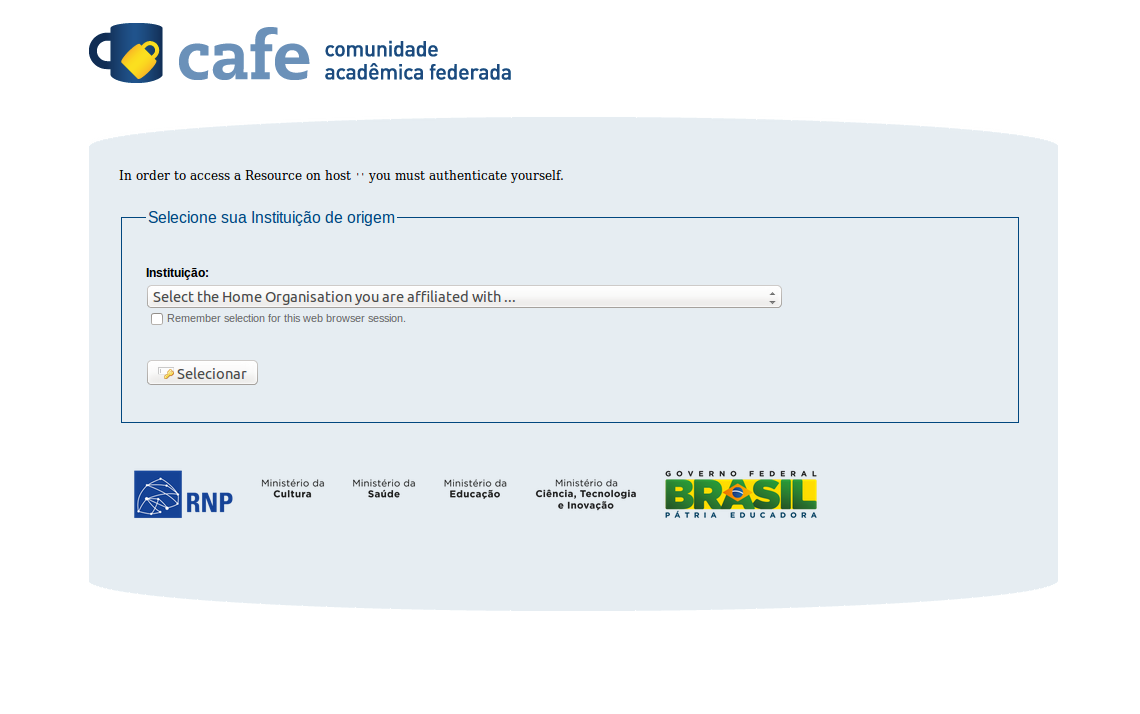
\includegraphics[scale=0.3]{images/escolher-federacao.png}
     \caption{Escolha de Federação}
     \label{fig:ufxc}
\end{figure}

\begin{figure}[ht]
     \centering
     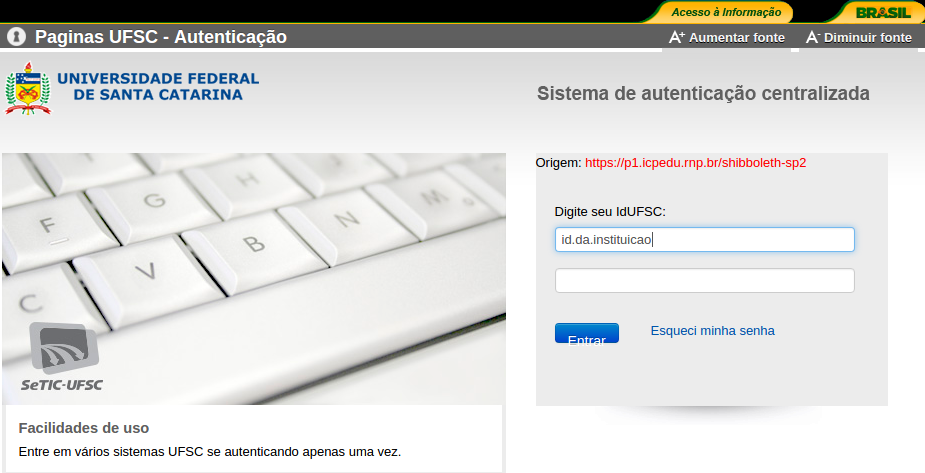
\includegraphics[scale=0.3]{images/emitir2.png}
     \caption{Autenticação na Federação}
     \label{fig:ufxc2}
\end{figure}

Se você já possui um certificado emitido nesta Autoridade Certificadora, e este ainda estiver ativo, um erro aparecerá na tela solicitando que o usuário confirme a emissão de um novo certificado digital, ou cancele a solicitação do mesmo.

Confirme que você deseja emitir um novo certificado em seu nome. A partir desta confirmação, o usuário verá uma tela com seus dados (Nome, CPF, E-mail e Data de  nascimento), onde nenhum deles pode ser editado. Basta conferir os dados e submeter a solicitação de certificado. Vide figura \ref{fig:emissao3}.

Quando o certificado for emitido, no canto superior esquerdo da tela aparecerá uma opção para visualizar o certificado (suas informações, detalhes e OIDs). Ao visualizar o certifica digital emitido, é possível conferir os dados gerais do certificado, em sua aba principal (imagem \ref{fig:geralcert}), e os detalhes do mesmo, em sua aba \textit{Details} (imagem \ref{fig:detailscert}).

\begin{figure}[ht]
     \centering
     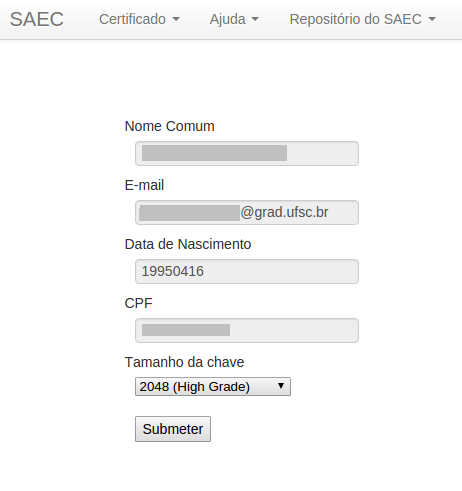
\includegraphics[scale=0.5]{images/emitir3.png}
     \caption{Confirmação de dados}
     \label{fig:emissao3}
\end{figure}

\begin{figure}[ht]
     \centering
     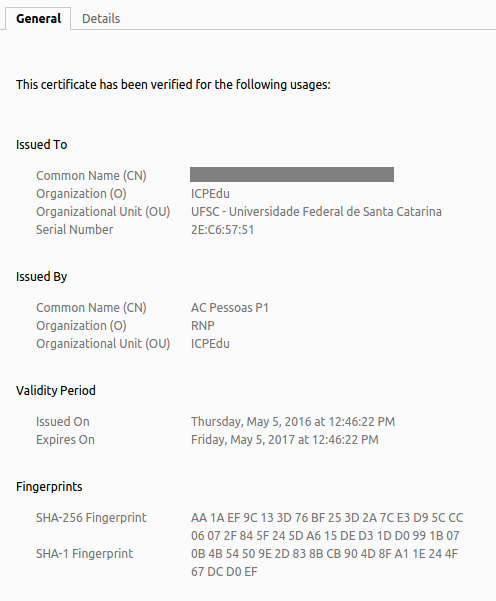
\includegraphics[scale=0.5]{images/geralcert.png}
     \caption{Informações gerais do certificado}
     \label{fig:geralcert}
\end{figure}

\begin{figure}[ht]
     \centering
     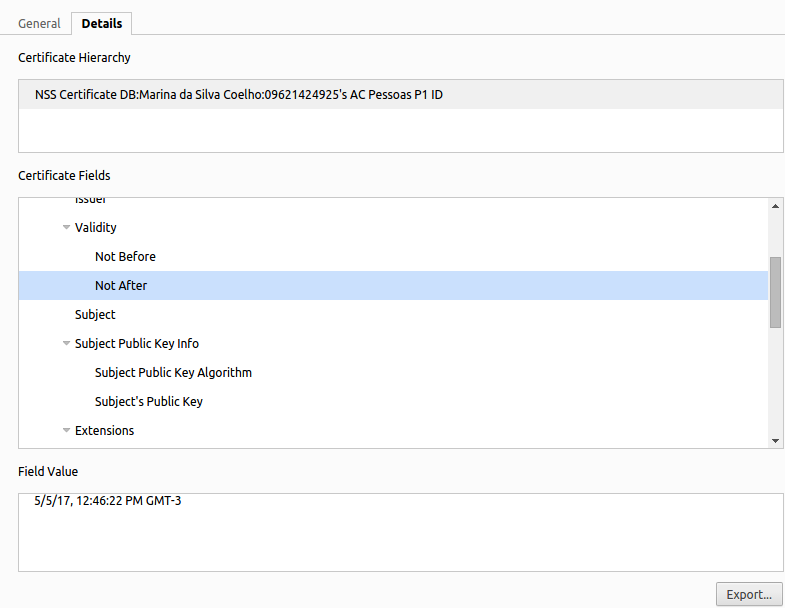
\includegraphics[scale=0.5]{images/details.png}
     \caption{Detalhes do certificado}
     \label{fig:detailscert}
\end{figure}

Como é possível ver na imagem \ref{fig:detailscert}, no canto inferior direito da tela de visualização de certificado, pode-se exportar o mesmo. A etapa para exportar o certificado envolve gerenciamento da chave do mesmo. Como este tipo de configuração é diferente para cada navegador (que também operam de maneira diferente dependendo do sistema operacional da máquina), o usuário deve se dirigir ao menu de ajuda, especificado na seção 7.2, onde poderá encontrar um guia detalhado de como exportar o certificado com base no navegador e sistema operacional utilizados no momento da exportação.

\section{Ajuda}

No menu \textit{Ajuda} é possível encontrar um guia que demonstra o passo a passo para todas as atividades do sistema, desde emissão do seu próprio certificado digital, até a configuração do cliente de e-mail. Basta clicar no menu e seguir as dicas da página.

\section{Repositório}

No menu \textit{Repositório do SAEC} é possível encontrar o certificado da Autoridade Certificadora, que será automaticamente instalado no caso de o usuário utilizar o navegador Mozilla Firefox, ou precisa ser manualmente instalado, caso o usuário use Google Chrome, Internet Explorer ou Safari. Para acessar o guia de instalação, basta clicar no link \textit{Ajuda com a instalação}, posicionado ao lado do certificado a ser baixado.

É possível também baixar a Lista de Certificados Revogados (LCR) da AC. Para instalar a LCR, é necessário, novamente, clicar no link \textit{Ajuda com a instalação}, disponibilizado ao lado da LCR. Ambos os links de ajuda redirecionarão o usuário para a página de ajuda, apresentada na seção 7.2.

 

\renewcommand\bibname{Referências}
\bibliographystyle{packages/abnt-num}
\bibliography{bibliografia}

\end{document}

